\chapter{Data}\label{ch:style}

\section{TMK Dataset}
The TMK dataset was created by Goldsmith, Butcher, Benjamin, Sowmya, Muchlinski (2020) in  \emph{“Introducing The Targeted Mass Killing Dataset for the Study and Forecasting of Mass Atrocities”}
The TMK dataset was created to contribute to the study into various atrocities such as genoicide, politicide. The dataset records events from 1946-2019 and tracks a wide variety of socioeconomic factors. The scale of the TMK event is quantified via a pre-coded ordinal indicator that aggregates evidence of intent as well as number of deaths.

\begin{center}
 \begin{tabular}{||c c c||} 
 \hline
 Score & Intent & Total Deaths\\ [1ex] 
 \hline
 1 & NO Stated OR Organizational Intent & $25 \leq x \leq 999$ \\ [1ex] 
 \hline
 2 & NO Stated OR Organizational Intent &  $\geq 1000$  \\ [1ex] 
 \hline
 3 & Stated OR Organizational Intent & $25 \leq x \leq 999$ \\ [1ex]  
 \hline
  & TMK GENOCIDE/POLITICIDE THRESHOLD & \\
 \hline
 4 & Stated AND Organizational Intent  &  $\geq 1000$  \\ [1ex] 
 \hline
  5 & Stated AND Organizational Intent  & $25 \leq x \leq 999$  \\ [1ex] 
 \hline
  6 & Stated AND Organizational Intent  &  $\geq 1000$   \\ [1ex] 
 \hline
  7 & Stated AND Organizational Intent  &  $\geq 10,000$   \\ [1ex] 
 \hline
  8 & Stated AND Organizational Intent  &  $\geq 100,000$   \\ [1ex] 
 \hline
\end{tabular}
\end{center}

\section{Alternative Data Sources}
\subsection{Social Conflict Analysis Database}
\subsection{Uppsala Conflict Data Program}
\section{Political Instability Task Force}
web-pages~\cite{Noo05}.  The requirements below are for the written thesis
only.


\section{Data Issues}
\subsection{Class Imbalance}
\subsection{Missing Values}
Like most datasets in social science a lot of events have missing values

\begin{figure}[h]
\caption{Proportion of missing values in TMK dataset}
\centering
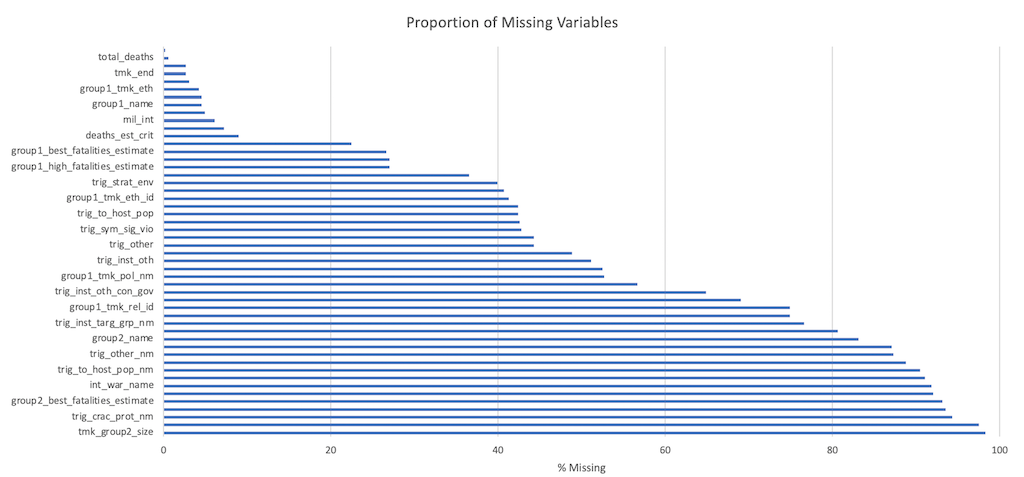
\includegraphics{proportionOfMissingvalues.png}
\end{figure}

\subsubsection{Logical Imputations}
Logical imputation involves replacing missing values when the logic is obvious. For example, missing values can be logically imputated for TMK related because the dataset contains only TMK events.

\subsubsection{Multivariate Imputation Chained Equations}
Multivariate Imputation via Chained Equations (MICE) comprises of two techniques as outlined by Van Buren (2018). The database contains missing values that match a \emph{"general pattern of missing data"}. 

MICE implements two methods for imputation of missing values. The first is Joint Modelling(JM) where imputations are drawn from a multivariate model fitted to data. The second is Fully Conditional Specification (FCS) involves drawing imputations from iterated conditional models. 

Both JM and FCS are available in R via the MICE package. A limitation of using the MICE package is that it can affect the bias and standard error of the data.

\begin{figure}[h]
\caption{General pattern of missing data visualized. Missing data in red}
\centering
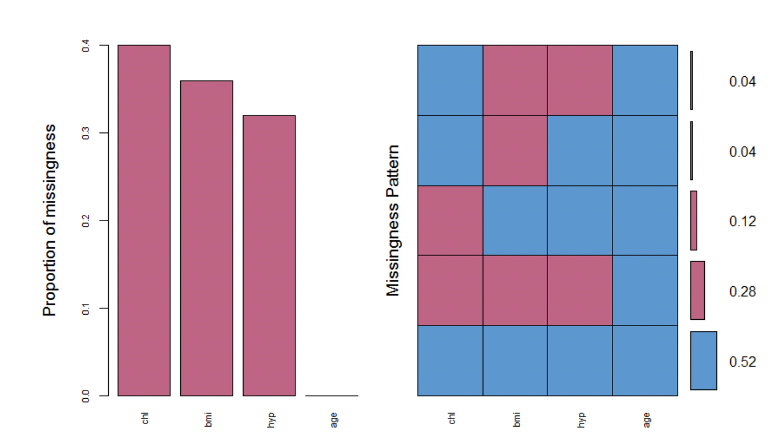
\includegraphics{missingdataimage.png}
\end{figure}



\subsection{Feature Explosion}
The TMK dataset already contains 121 different features. When additional datasets are merged via an outer join the number of features will only increase. When a model has to train on too many features it will encounter difficulty in identifying important features from less useful ones. This is known as the curse of dimensionality. 

To deal with the problem of feature explosion we will apply the Recursive Feature Elimination Algorithm(RFE) which is availability in the sklearn framework in python. 

As depicted here the RFE  algorithm recursively removes features at each step and re-ranks remaining features by retraining Support vector machines based on these remaining features. If a feature is a weak feature, RFE will simply remove it. this can be a problem, because a weak feature may still be an important feature when used in conjunction with other features this will be something I will have to take into account



